
\subsection{Qué es question answering}


\begin{frame}
  \frametitle{¿Qué es question answering?}
  \begin{block}{Question Answering}<1->
      Es el proceso automatizado de generación de respuestas concretas para preguntas formuladas en lenguaje natural.
  \end{block}
  \bigskip

 \begin{alertblock}{Question}<2->
      ¿Quién desarrolló la teoría de la relatividad?
  \end{alertblock}

  \begin{columns}<2->
      \begin{column}{.5\textwidth}
      \end{column}
      \begin{column}{.1\textwidth}
      \begin{tikzpicture}[>=stealth, rotate border/.style={shape border uses incircle, shape border rotate=270}]
              \node[rotate border=-40, fill=black, minimum height=1.5cm, single arrow, single arrow head extend=.3cm, single arrow head indent=.1cm, inner sep=1.5pt] (arrow) {};
          \end{tikzpicture}
      \end{column}
      \begin{column}{.3\textwidth}
          %Question Answering
      \end{column}
      \begin{column}{.5\textwidth}

      \end{column}
  \end{columns}

  \begin{exampleblock}{Answer}<2->
      Albert Einstein.
  \end{exampleblock}
\end{frame}


\begin{frame}
\frametitle{Ejemplo IR: esto no es QA}
\begin{figure}
  \centering
    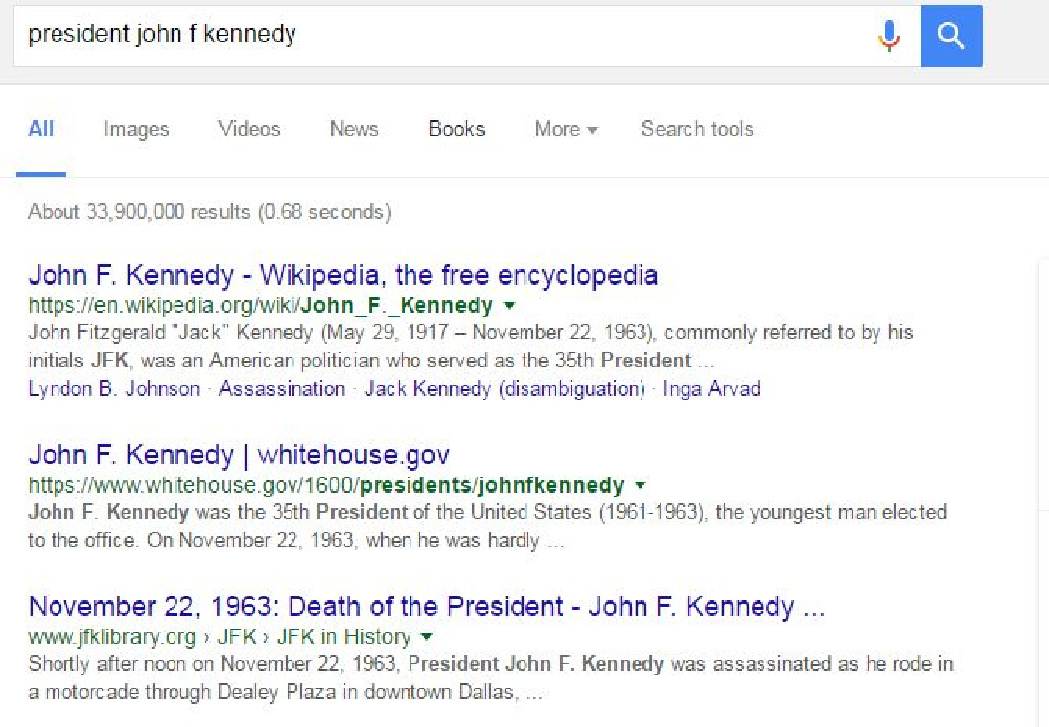
\includegraphics[scale=.4]{graficos/i-r-example}
  \caption{Google como sistema de Information Retrieval \newline \tiny{IR es: \dq{retornar \textit{información relevante} para una \textit{consulta} (\textit{information need}) a partir de una \textit{base de conocimiento}}}}
  \label{fig:qa-example}
\end{figure}

\end{frame}


\begin{frame}
\frametitle{Ejemplo QA: esto es QA}
\begin{figure}
  \centering
    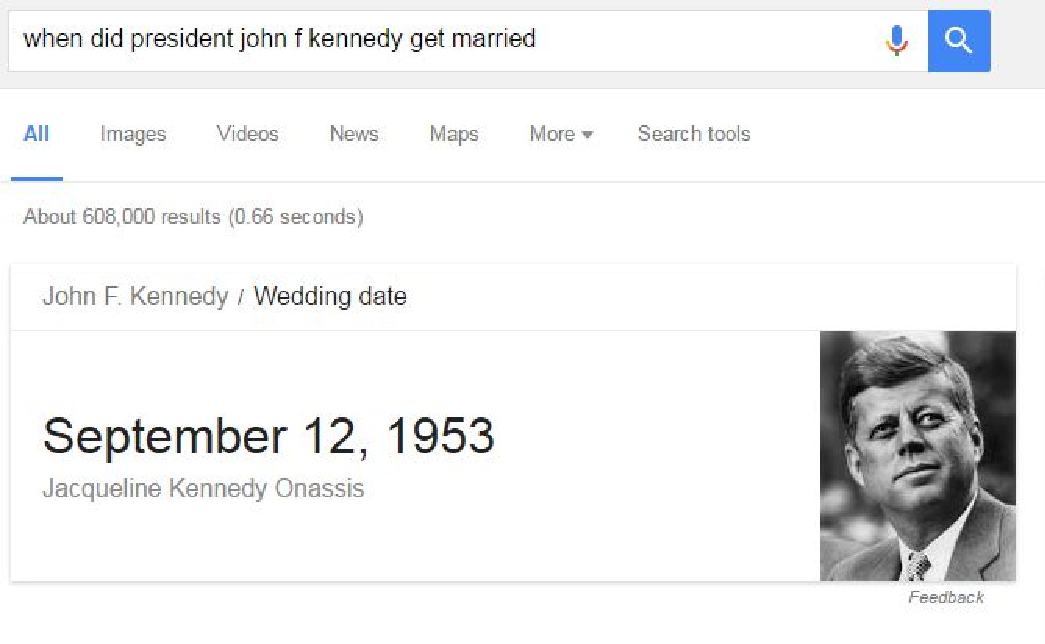
\includegraphics[scale=.5]{graficos/q-a-example}
  \caption{Google como sistema de Question Answering \newline \tiny{QA es IR, pero más específico en qué significa \textit{consulta} y qué significa \textit{información relevante}}}
  \label{fig:qa-example}
\end{figure}
  
\end{frame}


\begin{frame}
  \frametitle{Ejes de clasificación}
  \begin{block}{Generalidad del dominio}
    Dominio abierto o dominio cerrado
    \begin{itemize} 
      \item Enciclopedias, Internet
      \item Restaurants, clima, transportes.
    \end{itemize}
  \end{block}


  \begin{block}{Tipo de datos}
    \begin{itemize}
      \item Estructurado / no estructurado.
      \begin{itemize}
          \item Bases de datos, texto plano, texto formateado.
      \end{itemize}
    \end{itemize}
  \end{block}
\end{frame}


\subsection{Qué es esta tesis}

\begin{frame}[<+->]\fontsize{11pt}{11}\selectfont
  \frametitle{Qué es esta tesis}
    \begin{block}{Brevemente}
      Implementamos dos sistemas de question answering\newline(no, no hay hipótesis; es práctica)
    \end{block}
    \begin{exampleblock}{Dominio cerrado con soporte para inglés / Popescu World}
      \begin{itemize}
          \item Estructurado - Base de datos relacional: countries, cities, languages
          \item Modelo teórico de \textit{tratabilidad semántica}
          \item Traduce preguntas a consultas SQL
      \end{itemize}
    \end{exampleblock}
    \begin{alertblock}{Dominio abierto con soporte multilingüe / Multilingual Qanus}
      \begin{itemize}
          \item No estructurado - Wikipedia(s) como base de conocimientos.
          \item Framework Qanus adaptado para Freeling
          \item Basado en IR + NLP + heurísticas
      \end{itemize}
    \end{alertblock}
\end{frame}